\documentclass[tikz,14pt,fleqn]{article}

\setlength{\parskip}{0.5\baselineskip}%
\usepackage[utf8]{inputenc}
\usepackage[margin=1in]{geometry}
\usepackage[titletoc,title]{appendix}
\usepackage{latexsym}
\usepackage{amssymb}
\usepackage{gensymb}
\usepackage{amsmath}
\usepackage{mathrsfs}
\usepackage{amsfonts}
\usepackage[dvipsnames]{xcolor}
\usepackage{multicol}
\usepackage{graphicx}
\usepackage{animate}
\usepackage{fancyhdr}
\usepackage[linguistics]{forest}
\usepackage{colortbl}
\usepackage{pdfpages}
\usepackage{wrapfig}
\usepackage{cancel}
\usepackage{multirow}
\usepackage[export]{adjustbox}
\usepackage{subcaption}

\usepackage{minted}
\definecolor{LightGray}{gray}{0.95}
\setminted{
    frame=lines,
    framesep=2mm,
    baselinestretch=1.2,
    bgcolor=LightGray,
    fontsize=\small,
    linenos,
    mathescape=true,
    escapeinside=||,
    fontsize=\footnotesize,
}

\definecolor{darkblue}{rgb}{0.0, 0.0, 1}
\usepackage[pdftex,hyperfigures,hyperindex,bookmarksnumbered,colorlinks, bookmarks, breaklinks, linktocpage,citecolor=darkblue,urlcolor=darkblue,linkcolor=darkblue,pagebackref=true,linktoc=all]{hyperref}
\usepackage{cleveref}

% to fixme
\usepackage{xcolor} 
\definecolor{FIXMECOLOR}{rgb}{1,0,0}
\newcommand{\FIXME}[1]{{\color{FIXMECOLOR}{\textbf{FIXME: #1}}}} 

% to simplify math 

\newcommand{\bvec}[1]{
   \ensuremath{
   \begin{bmatrix}
       #1 \\
   \end{bmatrix}
}}

\newcommand{\bmat}[1]{
   \ensuremath{
   \begin{bmatrix}
       #1
   \end{bmatrix}
}}

\newcommand{\dotprod}[2]{\ensuremath{\left< #1, #2 \right>}}

%% For plotting
\usepackage{pgfplots}
\pgfplotsset{width=10cm,compat=1.9}
\usepgfplotslibrary{external}
\tikzexternalize
%%
\usepackage{dirtree}
\usepackage{subcaption}
\usepackage{xifthen}% provides \isempty test
\usepackage{glossaries}

\captionsetup[subfigure]{labelformat=empty}
\definecolor{color1}{HTML}{0B0C10}
\definecolor{color2}{HTML}{1F2833}
\definecolor{color3}{HTML}{C5C6C7}
\definecolor{color4}{HTML}{66FCF1}
\definecolor{color5}{HTML}{45A29E}

\pagestyle{fancy}
\fancyhf{}
%%%%%%%%%%%%%%%%%%%%%%%%%%%%
%% VARIABLES
\newcommand\namesurname{Albert Cerfeda, Alessandro Gobbetti}
\newcommand\assignment{Assignment 3 - Frequency Domain Processing}

\newcommand\subject{Image \& Video Processing}
\newcommand\documentdate{15 May 2023}

% Title content
%%%%%%%%%%%%%%%%%%%%%%%%%%%%
\rhead{\assignment}
\lhead{\namesurname}
%%%%%%%%%%%%%%%%%%%%%%%%%%%%

\rfoot{Page \thepage}


\begin{document}

\begin{titlepage}
   \begin{center}
       \vspace*{0.2cm}

       \textbf{\Large{\subject}}

       \vspace{0.5cm}
        \textbf{\assignment}\\[5mm]
        
            
       \vspace{0.4cm}

        \namesurname
        \begin{figure}[H]
            \centering
        \end{figure}
       \tableofcontents

       \vspace*{\fill}
     
        
\includegraphics[width=0.4\textwidth]{fig/logo.png}
       
        \documentdate \\
        Università della Svizzera italiana\\
        Faculty of Informatics\\
        Switzerland\\

   \end{center}
\end{titlepage}

\section{Theoretical exercise [2 points]}
In this section, we will show that if $f(x,y) = g(x)\cdot g(y)$, then the Fourier transform of $F(u,v) = G(u)\cdot G(v)$, where $G(u)$ is the Fourier transform of $g(x)$.\\
We know that a 2D Fourier transform is defined as:
$$F(u,v) = \int_{-\infty}^{\infty} \int_{-\infty}^{\infty} f(x,y) \cdot e^{-j2\pi(ux+vy)} dx dy$$

We can substitute $f(x,y)$ with $g(x)\cdot g(y)$:
$$F(u,v) = \int_{-\infty}^{\infty} \int_{-\infty}^{\infty} g(x)\cdot g(y) \cdot e^{-j2\pi(ux+vy)} dx dy$$

We can split the integral in two parts:
$$F(u,v) = \int_{-\infty}^{\infty} g(x) \cdot e^{-j2\pi ux} dx \cdot \int_{-\infty}^{\infty} g(y) \cdot e^{-j2\pi vy} dy$$

We can recognize the Fourier transform of $g(x)$ and $g(y)$:
$$F(u,v) = G(u) \cdot G(v)$$
Therefore we have shown that if $f(x,y) = g(x)\cdot g(y)$, then the Fourier transform of $F(u,v) = G(u)\cdot G(v)$.


\section{Theoretical exercise [2 points]}
We compute Fourier transform $G(\mu)$ of function $g(x) = f(x)+f(-x)$, where $f(x)$ is the function plotted in \autoref{fig:1a}.
The function $g(x)$ is plotted in \autoref{fig:1b}.
\begin{figure}[h]
    \centering
    \begin{subfigure}{0.48\linewidth}
        \centering
        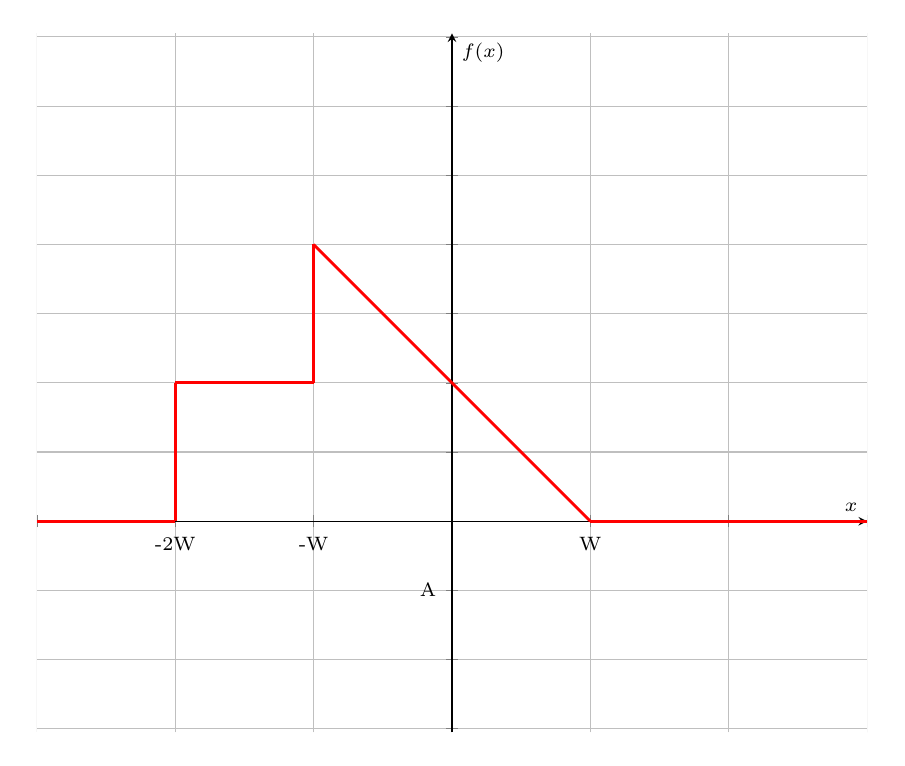
\begin{tikzpicture}
            \tikzstyle{every node}=[font=\scriptsize]
            \begin{axis}[
                axis lines=middle,
                % same axes scale
                grid=both,
                width=\textwidth,
                % height=0.5\textwidth, 
                % label style={font=\scriptsize},
                % tick label style={font=\tiny},
                xlabel={$x$},
                ylabel={$f(x)$},
                axis equal,
                ymin=-0.5,
                ymax=2.5,
                xmin=-3,
                xmax=3,
                % xticks={-2,-1,0,1,2},
                xticklabels={,,-2W,-W,,W,},
                yticklabels={,,,A,2A},
                ]
                \addplot[thick, samples=100, color=red, line width=1pt] coordinates {(-3,0)(-2,0)};
                \addplot[thick, samples=100, color=red, line width=1pt] coordinates {(-2,0)(-2,1)};
                \addplot[thick, samples=100, color=red, line width=1pt] coordinates {(-2,1)(-1,1)};
                \addplot[thick, samples=100, color=red, line width=1pt] coordinates {(-1,1)(-1,2)};
                \addplot[thick, samples=100, color=red, line width=1pt] coordinates {(-1,2)(1,0)};
                \addplot[thick, samples=100, color=red, line width=1pt] coordinates {(1,0)(3,0)};                
            \end{axis}
        \end{tikzpicture}
        \caption{Spatial domain function $f(x)$.}  
        \label{fig:1a}      
    \end{subfigure}    
    \begin{subfigure}{0.48\linewidth}
        \centering
        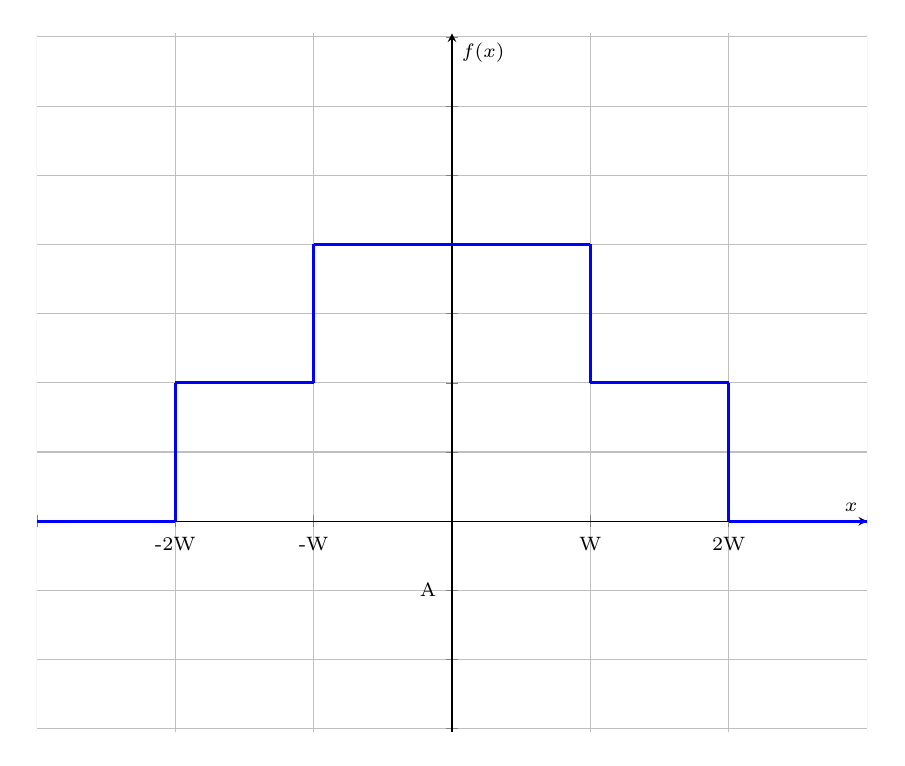
\begin{tikzpicture}
            \tikzstyle{every node}=[font=\scriptsize]
            \begin{axis}[
                axis lines=middle,
                % same axes scale
                grid=both,
                width=\textwidth, 
                % height=0.5\textwidth, 
                % label style={font=\scriptsize},
                % tick label style={font=\tiny},
                xlabel={$x$},
                ylabel={$f(x)$},
                axis equal,
                ymin=-0.5,
                ymax=2.5,
                xmin=-3,
                xmax=3,
                % xticks={-2,-1,0,1,2},
                xticklabels={,,-2W,-W,,W,2W},
                yticklabels={,,,A,2A},
                ]
                % g(x) = f(x) + f(-x)
                \addplot[thick, samples=100, color=blue, line width=1pt] coordinates {(-3,0)(-2,0)};
                \addplot[thick, samples=100, color=blue, line width=1pt] coordinates {(-2,0)(-2,1)};
                \addplot[thick, samples=100, color=blue, line width=1pt] coordinates {(-2,1)(-1,1)};
                \addplot[thick, samples=100, color=blue, line width=1pt] coordinates {(-1,1)(-1,2)};
                \addplot[thick, samples=100, color=blue, line width=1pt] coordinates {(-1,2)(1,2)};
                \addplot[thick, samples=100, color=blue, line width=1pt] coordinates {(1,2)(1,1)};
                \addplot[thick, samples=100, color=blue, line width=1pt] coordinates {(1,1)(2,1)};
                \addplot[thick, samples=100, color=blue, line width=1pt] coordinates {(2,1)(2,0)};
                \addplot[thick, samples=100, color=blue, line width=1pt] coordinates {(2,0)(3,0)};
            \end{axis}
        \end{tikzpicture}
        \caption{Spatial domain function $g(x) = f(x) + f(-x)$.}
        \label{fig:1b}
    \end{subfigure}

    
    \caption{Spatial domain function $f(x)$ [red] and $g(x) = f(x) + f(-x)$ [blue].}
    \label{fig:1}
\end{figure}


By looking at \autoref{fig:1b}, it can be seen that the function $g(x)$ can be represented as the sum of two box functions.
\autoref{fig:2} shows the two box functions $h_1(x)$ and $h_2(x)$ that sum up to $g(x)$.

\begin{figure}[h]
    \centering
    \begin{subfigure}{0.48\linewidth}
        \centering
        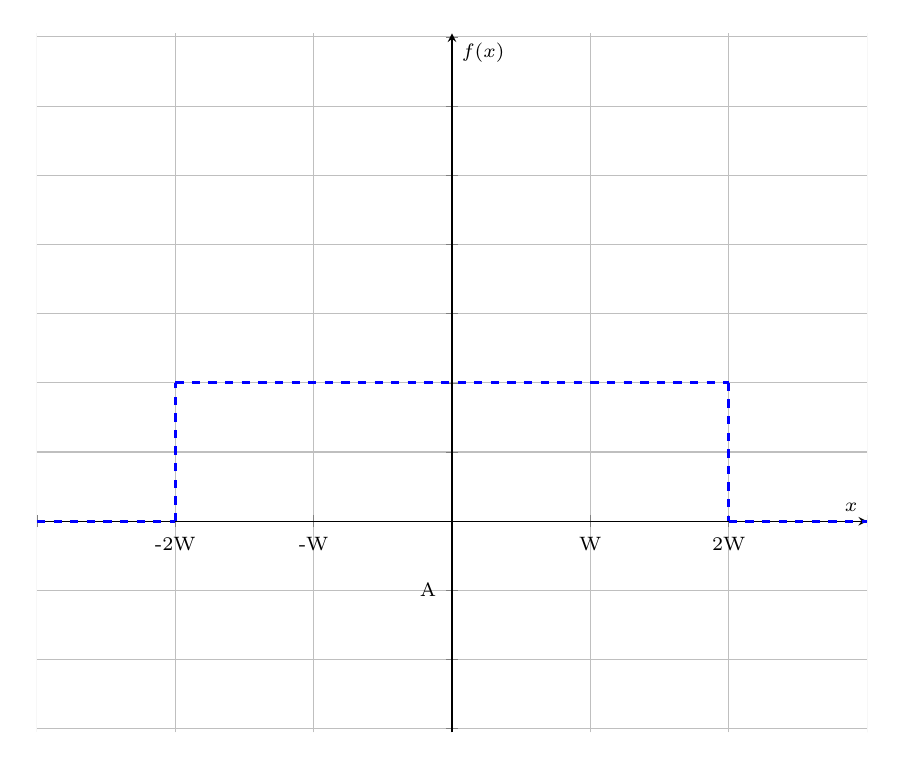
\begin{tikzpicture}
            \tikzstyle{every node}=[font=\scriptsize]
            \begin{axis}[
                axis lines=middle,
                % same axes scale
                grid=both,
                width=\textwidth,
                % height=0.5\textwidth, 
                % label style={font=\scriptsize},
                % tick label style={font=\tiny},
                xlabel={$x$},
                ylabel={$f(x)$},
                axis equal,
                ymin=-0.5,
                ymax=2.5,
                xmin=-3,
                xmax=3,
                % xticks={-2,-1,0,1,2},
                xticklabels={,,-2W,-W,,W,2W},
                yticklabels={,,,A,2A},
                ]
                \addplot[thick, samples=100, color=blue, line width=1pt, dashed] coordinates {(-3,0)(-2,0)};
                \addplot[thick, samples=100, color=blue, line width=1pt, dashed] coordinates {(-2,0)(-2,1)};
                \addplot[thick, samples=100, color=blue, line width=1pt, dashed] coordinates {(-2,1)(2,1)};
                % \addplot[thick, samples=100, color=blue, line width=1pt] coordinates {(-1,1)(-1,2)};
                % \addplot[thick, samples=100, color=blue, line width=1pt] coordinates {(-1,2)(1,2)};
                % \addplot[thick, samples=100, color=blue, line width=1pt] coordinates {(1,2)(1,1)};
                % \addplot[thick, samples=100, color=blue, line width=1pt] coordinates {(1,1)(2,1)};
                \addplot[thick, samples=100, color=blue, line width=1pt, dashed] coordinates {(2,1)(2,0)};
                \addplot[thick, samples=100, color=blue, line width=1pt, dashed] coordinates {(2,0)(3,0)};
            \end{axis}
        \end{tikzpicture}
        \caption{Box function $h_1(x)$.}  
        \label{fig:2a}      
    \end{subfigure}    
    \begin{subfigure}{0.48\linewidth}
        \centering
        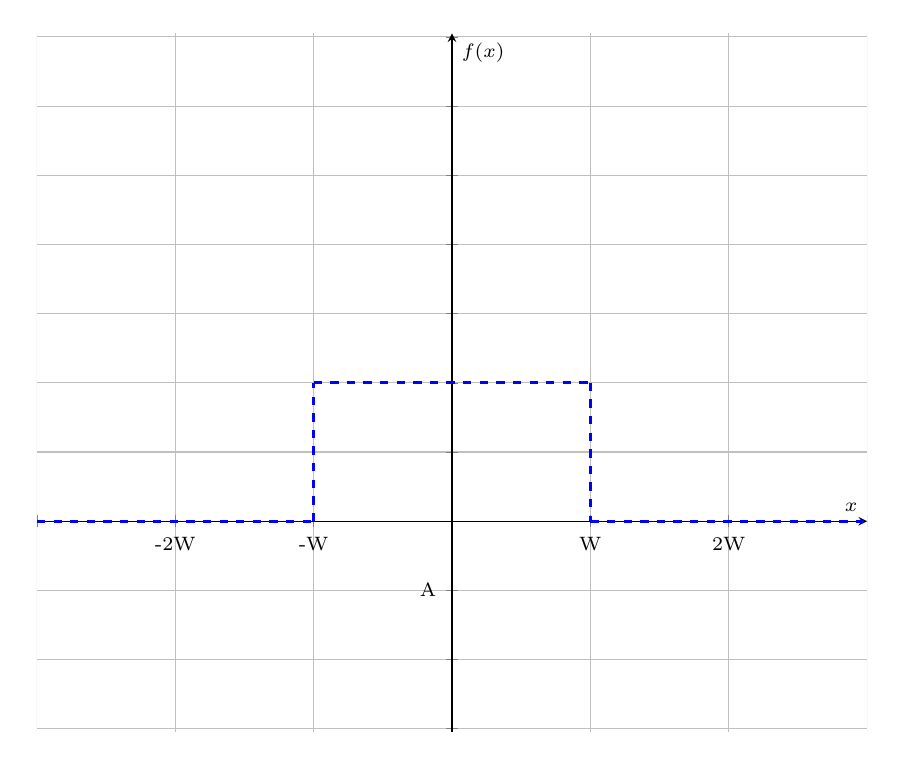
\begin{tikzpicture}
            \tikzstyle{every node}=[font=\scriptsize]
            \begin{axis}[
                axis lines=middle,
                % same axes scale
                grid=both,
                width=\textwidth, 
                % height=0.5\textwidth, 
                % label style={font=\scriptsize},
                % tick label style={font=\tiny},
                xlabel={$x$},
                ylabel={$f(x)$},
                axis equal,
                ymin=-0.5,
                ymax=2.5,
                xmin=-3,
                xmax=3,
                % xticks={-2,-1,0,1,2},
                xticklabels={,,-2W,-W,,W,2W},
                yticklabels={,,,A,2A},
                ]
                % g(x) = f(x) + f(-x)
                \addplot[thick, samples=100, color=blue, line width=1pt, dashed] coordinates {(-3,0)(-1,0)};
                % \addplot[thick, samples=100, color=blue, line width=1pt] coordinates {(-2,0)(-2,1)};
                % \addplot[thick, samples=100, color=blue, line width=1pt] coordinates {(-2,1)(-1,1)};
                \addplot[thick, samples=100, color=blue, line width=1pt, dashed] coordinates {(-1,0)(-1,1)};
                \addplot[thick, samples=100, color=blue, line width=1pt, dashed] coordinates {(-1,1)(1,1)};
                \addplot[thick, samples=100, color=blue, line width=1pt, dashed] coordinates {(1,1)(1,0)};
                % \addplot[thick, samples=100, color=blue, line width=1pt] coordinates {(1,1)(2,1)};
                % \addplot[thick, samples=100, color=blue, line width=1pt] coordinates {(2,1)(2,0)};
                \addplot[thick, samples=100, color=blue, line width=1pt, dashed] coordinates {(1,0)(3,0)};
            \end{axis}
        \end{tikzpicture}
        \caption{Box function $h_2(x)$.}
        \label{fig:2b}
    \end{subfigure}

    
    \caption{The two box functions that sum up to $g(x)$.}
    \label{fig:2}
\end{figure}

The Fourier transform of a box function $h(x)$ is known: $H(\mu) = AW\text{sinc}(\mu W)$, where $A$ is the amplitude of the box function
and $W$ is the width of the box.

We can thus express the Fourier transform of $g(x)$ as the sum of the Fourier transform of $h_1(x)$ and $h_2(x)$:
\begin{align*}
    G(\mu) &= H_1(\mu) + H_2(\mu) \\
    &= A4W\text{sinc}(\mu 4W) + A2W\text{sinc}(\mu 2W) \\
    &= A2W\left(2\text{sinc}(\mu 4W) + \text{sinc}(\mu 2W)\right)
\end{align*}
 



\section{Theoretical exercise} \label{sec:3}

Reducing the size of an image can lead to aliasing unless a low-pass filter is applied before.
The goal of this exercise is to find the smallest standard deviation of a Gaussian filter that can be applied in the spatial domain to avoid aliasing when reducing the size of an image by a factor of $c$.\\

When sampling, we make use of the \textit{Impulse signal} to take equally-spaced samples. The sample density is defined through the constant $\Delta T$. Reducing the size of an image by a factor of $c$ means that when performing downsampling we sample one pixel every $c$ pixels, i.e. $\Delta T = c$. It is important to note that the Fourier transform of an Impulse signal $s_{\Delta T}(t)$ with $\Delta T = c$  in the spatial domain results in another Impulse signal defined in the frequency domain $\mathscr{F}\{s_{\Delta T}(t)\}$with $\Delta T = \frac{1}{c}$. The translation from the spatial domain to the frequency (Fourier) domain can be visualized in \autoref{fig:4.impulse}:
% TODO: insert animated gif
\begin{figure}[H]
    \centering
    % \animategraphics[width=0.4\linewidth]{12}{./fig/gif/frame_}{0}{134}
    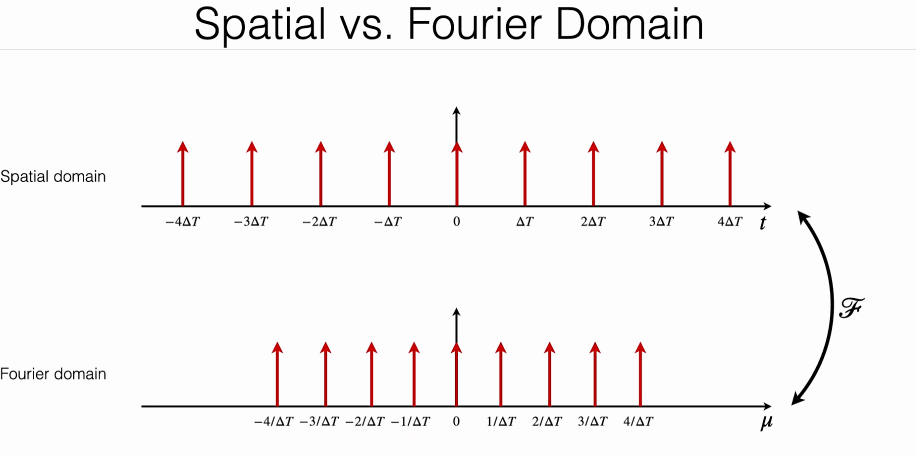
\includegraphics[width=0.4\linewidth]{./fig/3.spatialfourier.png}
    \caption{Equivalent Impulse signals in spatial and frequency domain}
    \label{fig:4.impulse}
\end{figure}

Convoluting the Fourier transformations of the image with an Impulse signal results in the image spectrum being repeated for every Impulse point in the Impulse train. If the Impulse train is too dense (i.e. $\Delta T$ is relatively small) the repeated image spectrums may overlap in certain positions. This leads to aliasing artifacts. This phenomenon is visualized in \autoref{fig:4.aliasing}.
\begin{figure}[H]
    \centering
    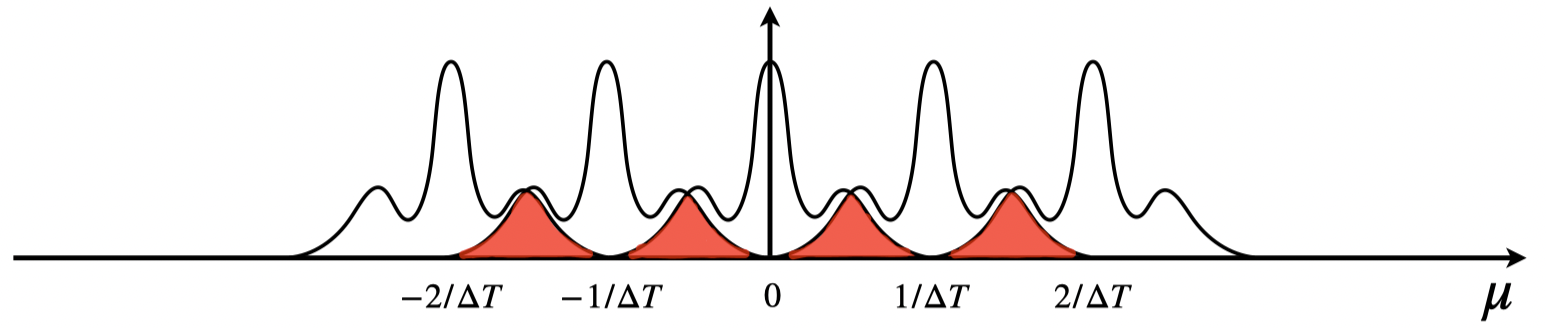
\includegraphics[width=0.8\linewidth]{fig/3.aliasing.png}
    \caption{$\mathscr{F}\left\{s_{\Delta T}(t)\right\} \star \mathscr{F}\{f(t)\}$}
    \label{fig:4.aliasing}
\end{figure}
As a countermeasure we apply Gaussian filtering on the image to get rid of high frequencies, resulting in the image spectrum being "narrower" and able to fit in the resulting spectrum without incurring overlaps.
We should thus find a Gaussian kernel that does not overlap in the frequency domain as shown in \autoref{fig:4.gaussian}.
\begin{figure}[H]
    \centering
    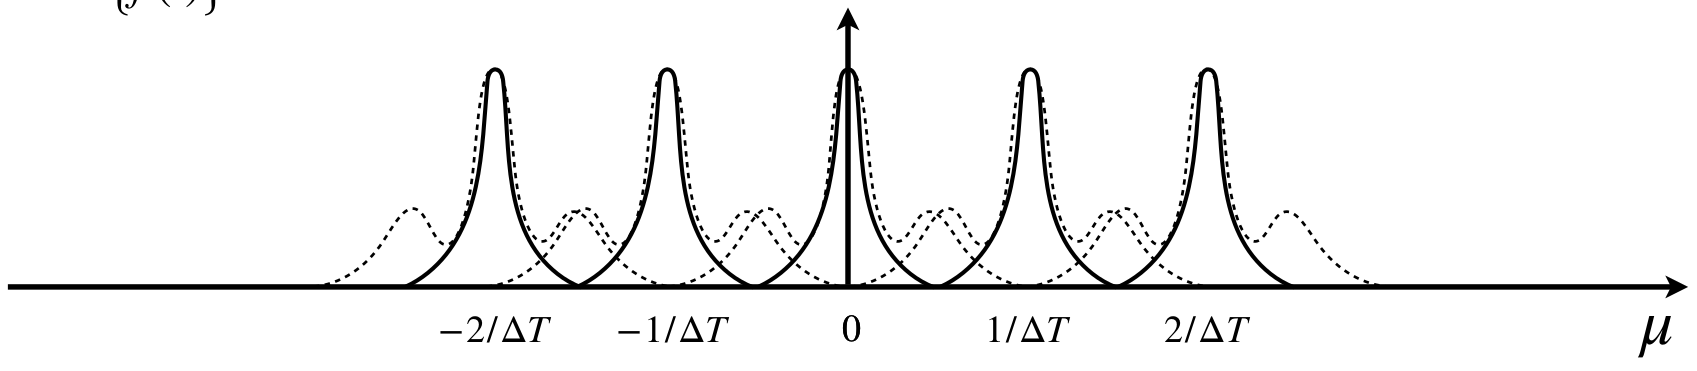
\includegraphics[width=0.8\linewidth]{fig/3.aliasing_gaussians.png}
    \caption{$\mathscr{F}\left\{s_{\Delta T}(t)\right\} \star \mathscr{F}\{f(t)\star g(t)\}$}
    \label{fig:4.gaussian}
\end{figure}


Given that $\Delta T = c$ is in the spatial domain, it is $\Delta T = \frac{1}{c}$ in the Fourier domain. We can use the size of the Gaussian kernel when performing prefiltering on the image to impose a bound on the width of the image spectrum in order not to incur into overlaps. 

However, a little bit of overlap is not a problem, for this exercise, we can assume that the spatial frequencies which are attenuated by a filter with a factor smaller than 0.75 do not cause aliasing.
We thus need to find the standard deviation $\sigma$ of the Gaussian kernel in the Fourier domain such that all the values are attenuated by a factor of at least 0.75.

From the Gaussian function:
\begin{equation*}
    G(x) = e^{-\frac12(\frac{x-\mu}{\sigma})^2},
\end{equation*}where $\mu$ is the mean and $\sigma$ is the standard deviation. 
We want then to find that $\sigma$ such that a Gaussian function with mean 0 and standard deviation $\sigma$ is attenuated by a factor of 0.75 at $x = \frac{1}{2c}$:
\begin{align*}
    0.75 = G(x) &= e^{-\frac12(\frac{x-0}{\sigma})^2} \\
    0.75 &= e^{-\frac12(\frac{x}{\sigma})^2} \\
    \ln(0.75) &= -\frac12(\frac{x}{\sigma})^2 \\
    \sigma^2 &= -\frac{x^2}{2\ln(0.75)} \\
    \sigma^2 &= -\frac{(\frac{1}{2c})^2}{2\ln(0.75)} \\
    \sigma &= \sqrt{-\frac{1}{8\ln(0.75)c^2}} \\
    \sigma &= \frac{1}{c}\sqrt{-\frac{1}{8\ln(0.75)}}\\
    \sigma &\approx \frac{0.66}{c}
\end{align*}

The standard deviation $\sigma$ found above is in the Fourier domain. To find the standard deviation $\sigma_s$ of the corresponding Gaussian kernel in the spatial domain (since the Fourier transform of a Gaussian function is another Gaussian function):
\begin{align*}
    \sigma_s&=\frac{1}{2\sigma \pi} \\
    \sigma_s&\approx\frac{1}{2\frac{0.66}{c} \pi} = \frac{c}{1.32\pi} \\
\end{align*}



\subsection{Bonus}
The Fourier transform of a Gaussian function $g(x) = e^{-x^2}$ is another Gaussian function.
\begin{align*}
    \mathscr{F}_x[g(x)](k) &= \int_{-\infty}^{+\infty}{g(x)e^{-2\pi kix}dx}\\
    &= \int_{-\infty}^{+\infty}{e^{-x^2}e^{-2\pi kix}dx}\\
    &= \int_{-\infty}^{+\infty}{e^{-x^2}[\cos(2\pi kx) - i\sin(2\pi kx)]dx}\\
    &= \int_{-\infty}^{+\infty}{e^{-x^2}\cos(2\pi kx)dx} - i\int_{-\infty}^{+\infty}{e^{-x^2}\sin(2\pi kx)dx}
\end{align*}
The integral of the imaginary part is zero since the integrand is an odd function and the integration interval is symmetric. We are left with the integral of the real part:
\begin{align*}
    \mathscr{F}_x[g(x)](k) &= \int_{-\infty}^{+\infty}{e^{-x^2}\cos(2\pi kx)dx} \\
    &= \sqrt{\pi}e^{-\pi^2k^2}
\end{align*}
which is still a Gaussian function. So the Fourier transform of a Gaussian function is another Gaussian function.




\section{Theoretical exercise}
\autoref{fig:ex4} shows the magnitude of the Fourier spectrum of a spatial signal $f(x)$, which is two boxes centered around the frequency $±\omega_0$. We want to find the spatial signal $f(x)$ assuming arbitrary boxes' width $W$ and height $A$.

\begin{figure}[H]
    \centering
    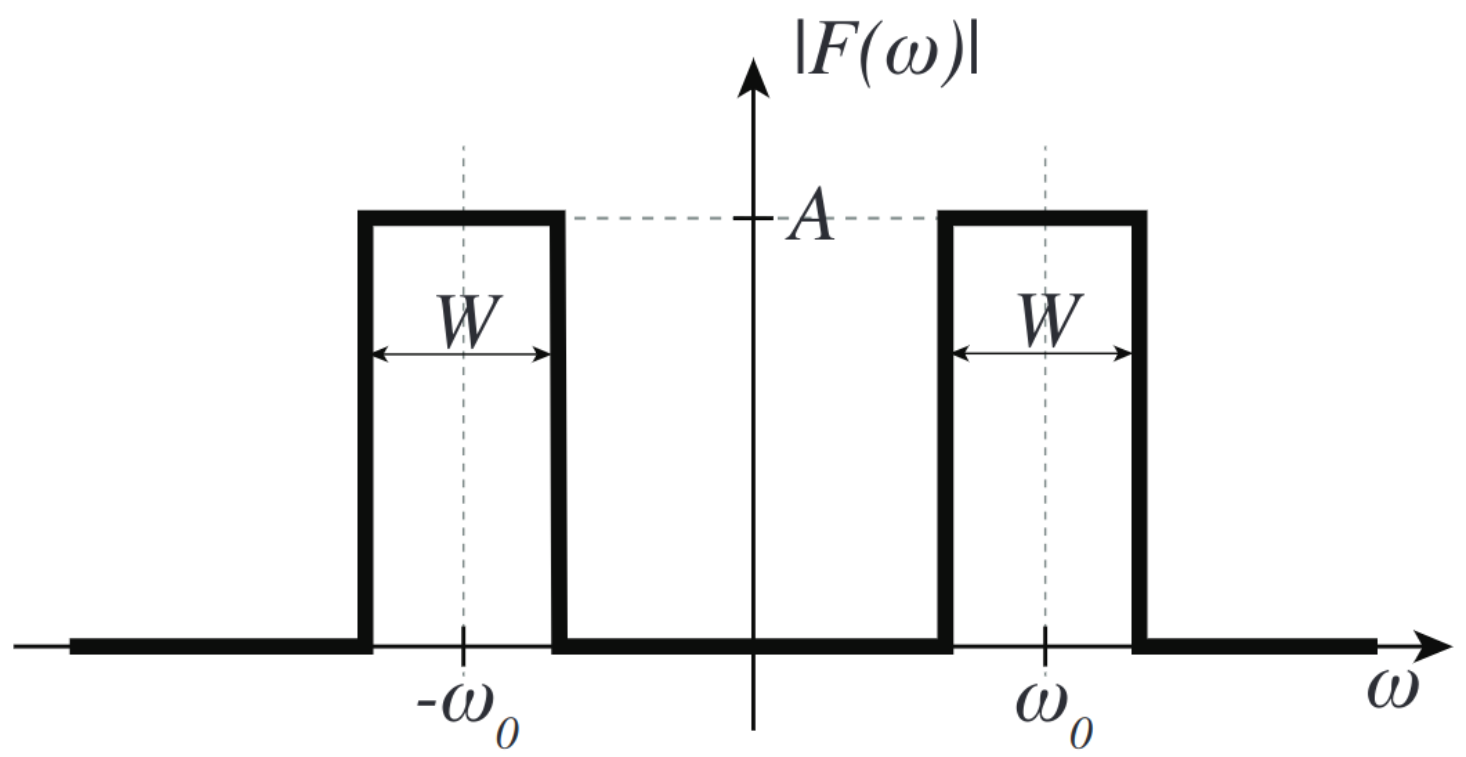
\includegraphics[width=0.4\linewidth]{fig/4.plot.png}
    \caption{Magnitude of the Fourier spectrum of a spatial signal $f(x)$.}
    \label{fig:ex4}
\end{figure}

% Looking at \autoref{fig:4}, we can notice two boxes centered around the frequency $±\omega_0$. Since the box function is the Fourier transform of a sinc function, we can state that the sinc function is part of $f(x)$. We also notice that the boxes are repeated at every multiple of $\omega_0$ in the frequency domain, therefore a sampling function seems to be part of $f(x)$ as well. 
% We also know from the convolution theorem that the Fourier transform of a convolution of two signals is a product of their Fourier transforms and vice versa.

Looking at \autoref{fig:ex4} we can identify multiple rect functions centered around the frequencies $±k\omega_0$. We can thus express the Fourier transform $F(x)$ as the convolution of a rect function $rect(x)$ and a sampling function $s_{\Delta T}(x)$:
\begin{equation*}
    F(x) = AW\texttt{rect}(Wx) \star s_{\omega_0}(x)
\end{equation*}
From the convolution theorem, we know that the Fourier transform of a convolution of two signals is a product of their Fourier transforms and vice versa.
We also know that the Fourier transform of a sinc function is a box function and that the Fourier transform of a sampling function is still a sampling function with a sampling period $\Delta T_f = \frac{1}{\Delta T_s}$.

The original signal $f(x)$ is then:
\begin{equation*}
    f(x) = AW\texttt{sinc}(WX) \cdot s_{\frac1{\omega_0}}(x)
\end{equation*}




\section{Theoretical exercise}
Consider a task of filtering a signal with a spatial domain Gaussian filter $h(x)$. 
The filter has been approximated with a kernel of inappropriate size ($s$), effectively windowing the original filter to $g(x)$.

The new filter has now a different Fourier transform than the original one ($G(\omega) \neq H(\omega)$), but it can be expressed as:
\begin{equation*}
    G(\omega) = H(\omega) \star X(\omega)
\end{equation*}
Our goal is to derive an expression for $X(\omega)$, where $s$ is an additional parameter.

\begin{figure}[H]
    \centering
    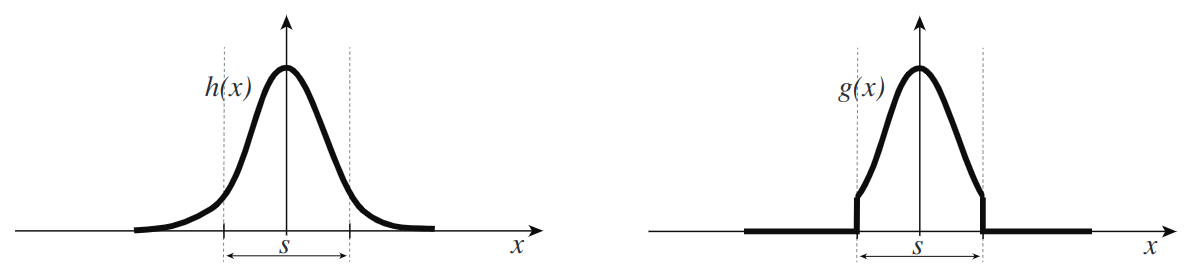
\includegraphics[width=0.8\linewidth]{fig/5.hx-gx.png}
    \caption{Visualization of the Gaussian filter $h(x)$ and its windowed version $g(x)$.}
    \label{fig:ex5}
\end{figure}

Looking at the windowed filter in \autoref{fig:ex5}, we can express $g(x)$ as the multiplication of the original filter and a box function of width $s$. The Fourier transform of a box function is a sinc function, therefore, recalling the fact that the product of two signals in the spatial domain is a convolution in the frequency domain, we can express $G(\omega)$ as:
\begin{equation*}
    G(\omega) = H(\omega) \star (s\cdot\texttt{sinc}(\omega s))
\end{equation*}

\begin{figure}[H]
    \centering
    \begin{subfigure}{0.49\linewidth}
        \centering
        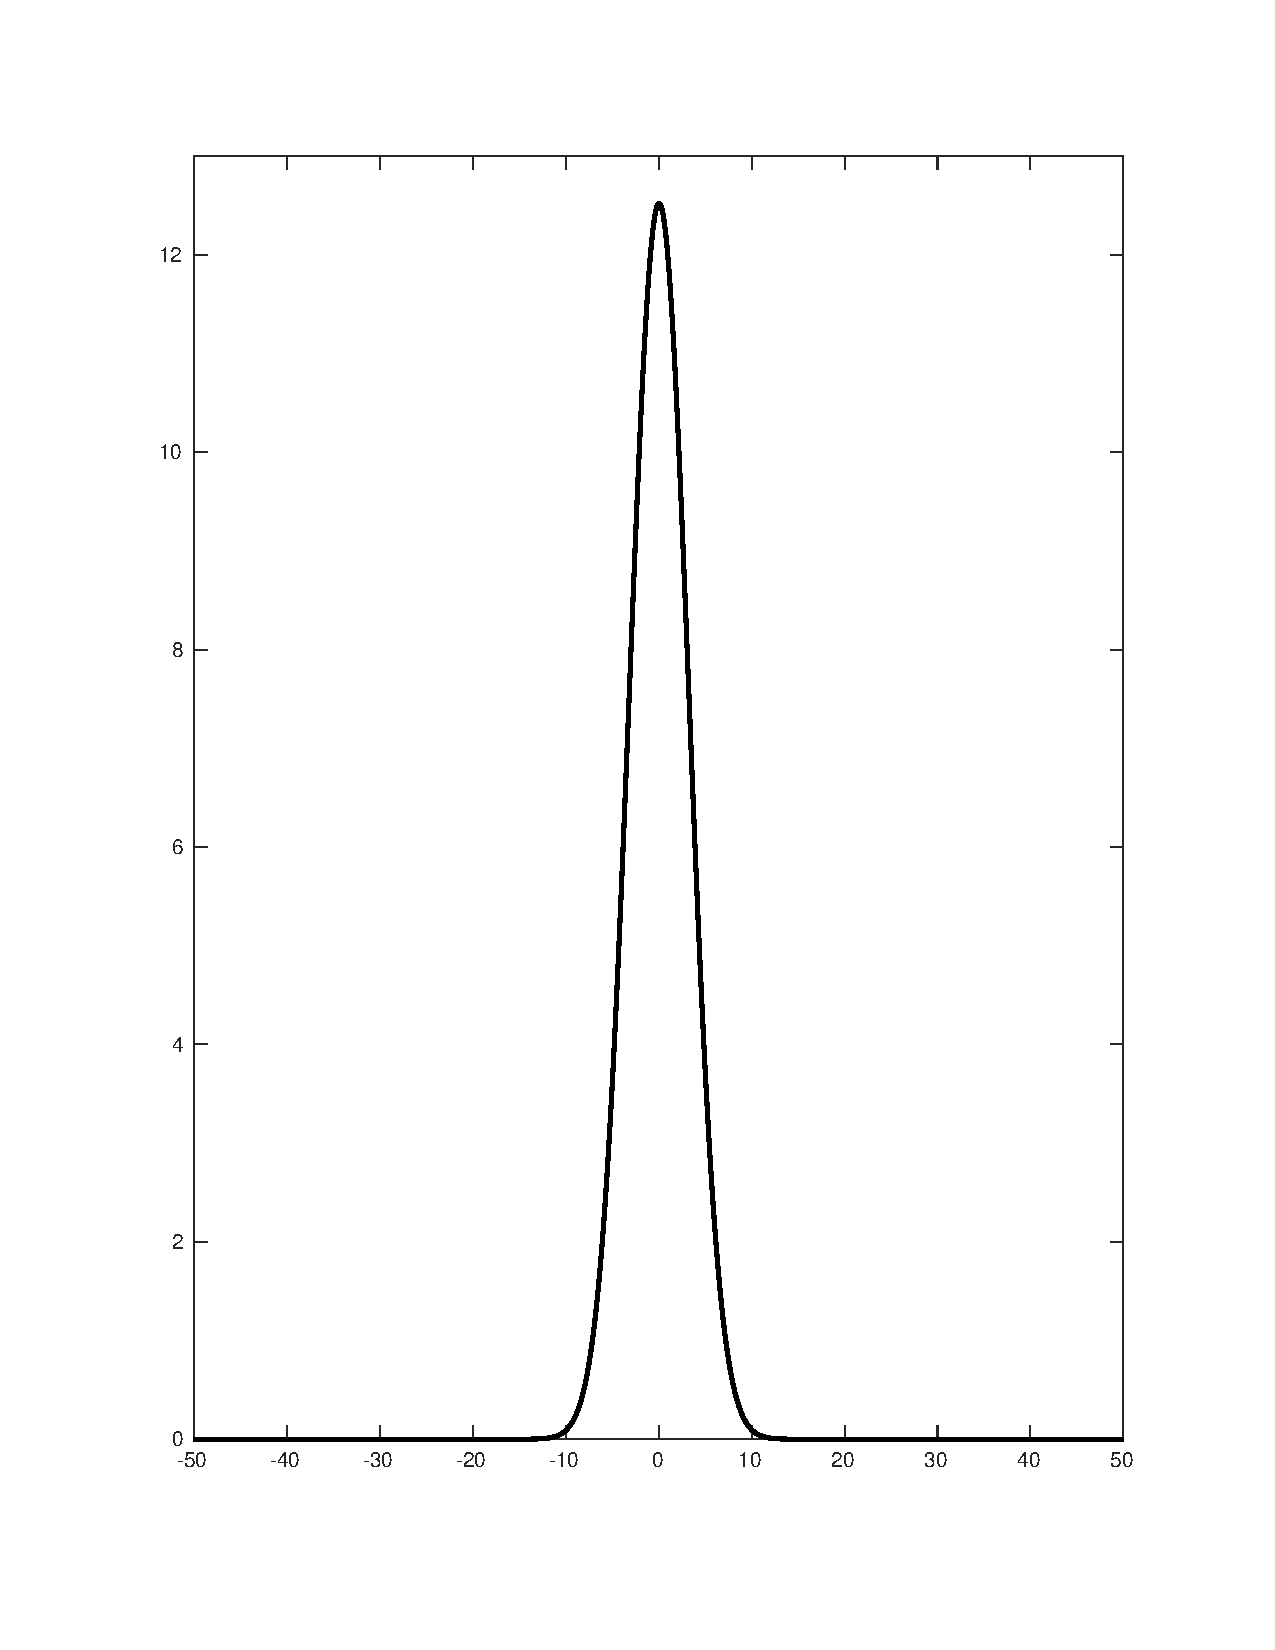
\includegraphics[width=\linewidth]{fig/out/5.hw.pdf}
        \caption{$H(\omega)$}
        \label{fig:ex5-Hw}
    \end{subfigure}
    \begin{subfigure}{0.49\linewidth}
        \centering
        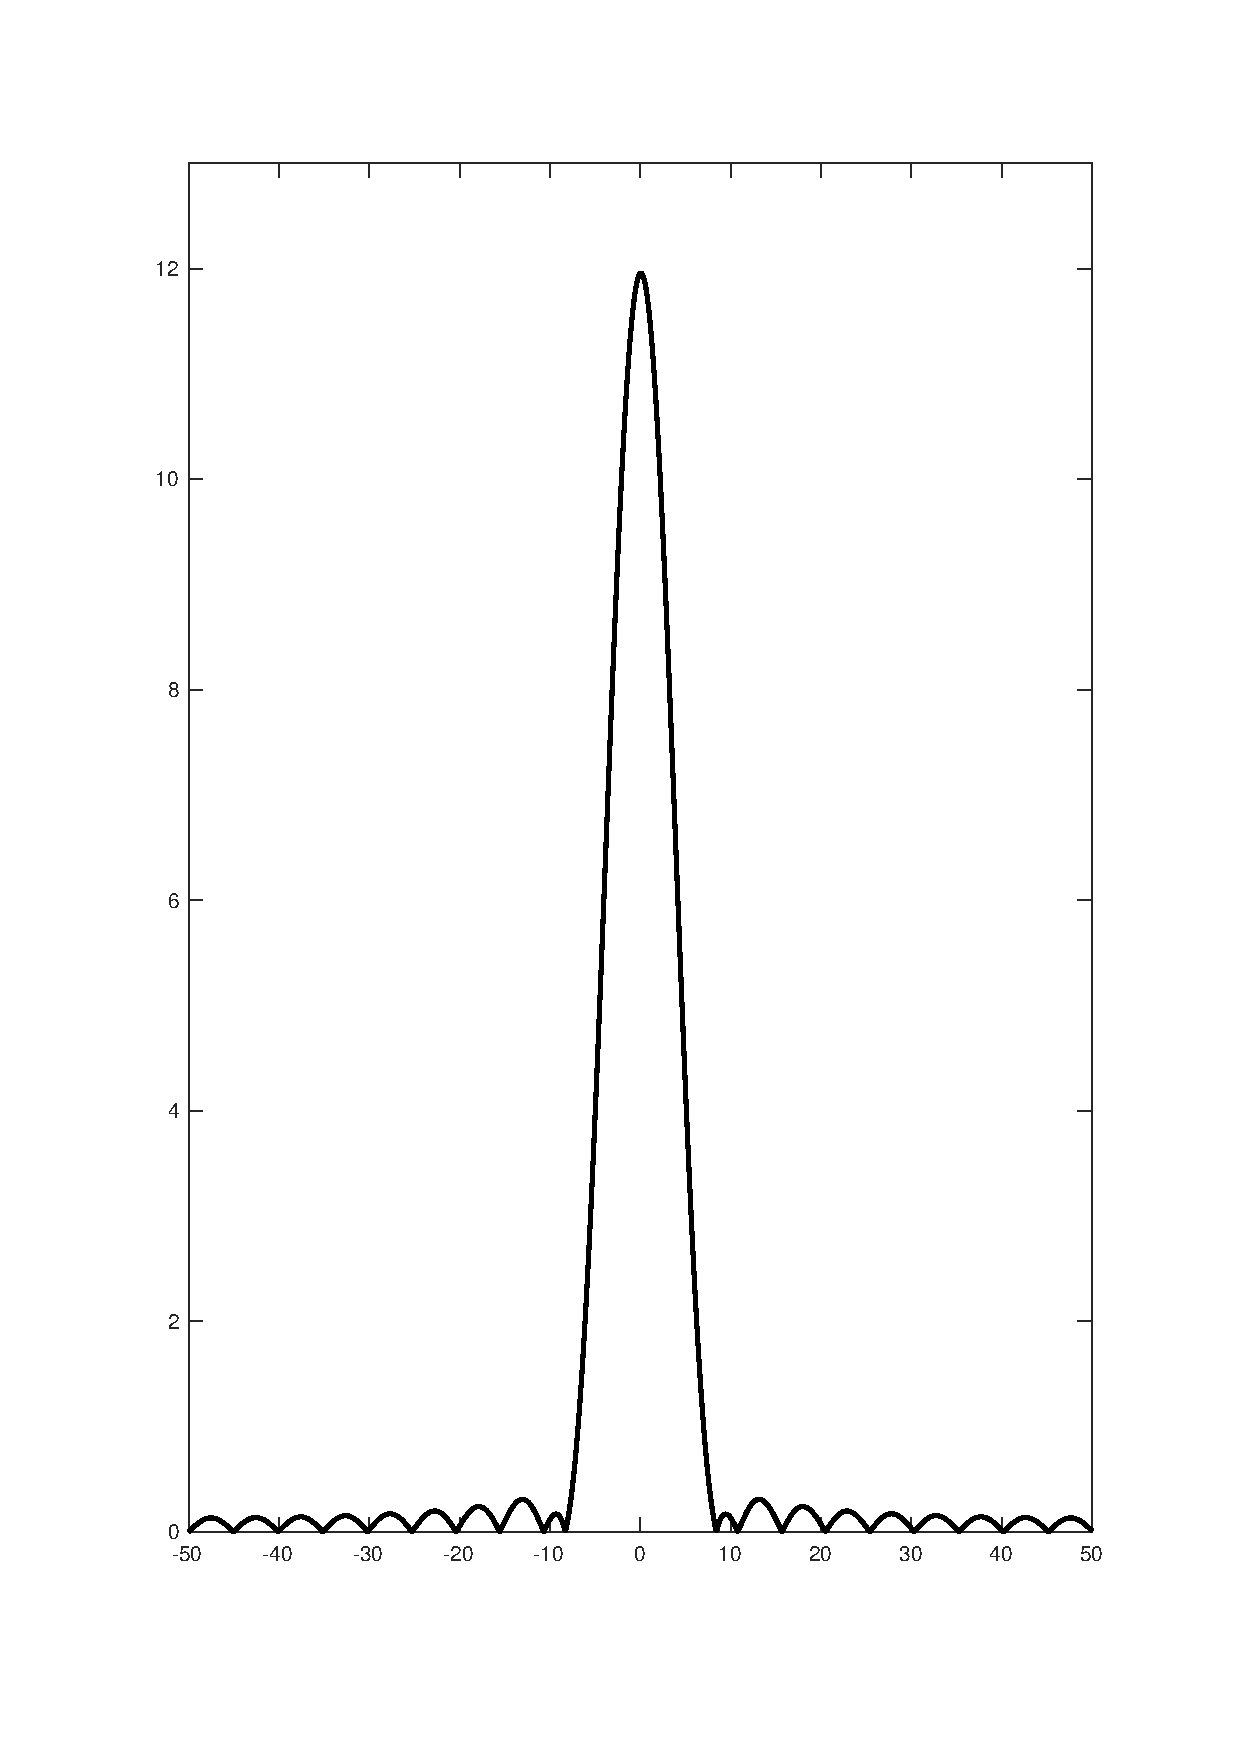
\includegraphics[width=\linewidth]{fig/out/5.gw.pdf}
        \caption{$G(\omega)$}
        \label{fig:ex5-Gw}
    \end{subfigure}
    \caption{Visualization of the Fourier transform of the Gaussian filter $H(\omega)$ and its windowed version $G(\omega)$.}
    \label{fig:ex5-Hw-Gw}
\end{figure}


In \autoref{fig:ex5-Hw-Gw} we can see the Fourier transform of the original Gaussian filter $H(\omega)$ and its windowed version $G(\omega)$. It can be seen that in $G(\omega)$ the convolution with the sinc function has the effect of amplifying some frequencies at the sides which were almost zero in the Gaussian version $H(\omega)$.

\clearpage 
\section{Gaussian Filtering [4 points]}
\subsection{Equivalence of spatial and frequency domain filtering}
In this exercise we have to implement Gaussian filtering both in the spatial and frequency domain. Namely, we want to show that convoluting a gaussian filter with $\sigma_s$ in the spatial domain is equivalent to performing point-wise multiplication in the fourier domain between the image spectrum and another gaussian filter with $\sigma_f = \frac{1}{2\sigma_s \pi}$.
\begin{itemize}
    \item \textbf{Spatial domain}
\begin{minted}[frame=lines, framesep=2mm, fontsize=\small ]{matlab} 
function [img_filtered] = spatialGaussianFiltering(img, sigma_s)
        kernel_size_s = 4*sigma_s+1;
        gaussian_filter_spatial = fspecial('gaussian', kernel_size_s, sigma_s);
        img_filtered = conv2(img,gaussian_filter_spatial,'same');
end
\end{minted}
Results are shown in \autoref{fig:ex6-spatial}.
    \item \textbf{Frequency domain}
\begin{minted}[frame=lines, framesep=2mm, fontsize=\small ]{matlab} 
function img2_filtered = frequencyGaussianFiltering(img, sigma_s)
    %%% Convert to frequency domain
    img2_fft = fft2(img);
    % Shift lower frequencies to the center of fourier spectrum
    img2_fft = fftshift(img2_fft);

    % Computing gaussian filter
    sigma_f = (1/(2*pi*sigma_s));
    [X,Y]= meshgrid(-size(img,1)/2:size(img,1)/2-1,-size(img,2)/2:size(img,2)/2-1);
    D = sqrt(X.^2 + Y.^2);
    D = D/max(D(:));
    D = exp(-D.^2/2/sigma_f^2);
    D = D/max(D(:));
    gaussian_filter_frequency = D;

    % Perform gaussian filtering in frequency domain
    img2_filtered_fft = img2_fft .* gaussian_filter_frequency;
    % Bring image back to spatial domain
    img2_filtered = ifft2(ifftshift(img2_filtered_fft));
end
\end{minted}
Results are shown in \autoref{fig:ex6-frequency}.
\end{itemize}


\begin{figure}[h!]
    \centering
    \begin{subfigure}{0.23\textwidth}
        \centering
        
\includegraphics[width=.7\textwidth]{fig/out/6.img.png}
        \caption{Original image}
    \end{subfigure}
    \begin{subfigure}{0.23\textwidth}
        \centering
        
\includegraphics[width=.7\textwidth]{fig/out/6.gaussian_filter_spatial.png}
        \caption{Spatial gaussian filter}
    \end{subfigure}
    \begin{subfigure}{0.23\textwidth}
        \centering
        
\includegraphics[width=.7\textwidth]{fig/out/6.img_filtered.png}
        \caption{Filtered image}
    \end{subfigure}
    \caption{Gaussian filtering pipeline in the spatial domain}
    \label{fig:ex6-spatial}
\end{figure}
\begin{figure}[h!]
    \centering
    \begin{subfigure}{0.32\textwidth}
        \centering
        
\includegraphics[width=.5\textwidth]{fig/out/6.img.png}
        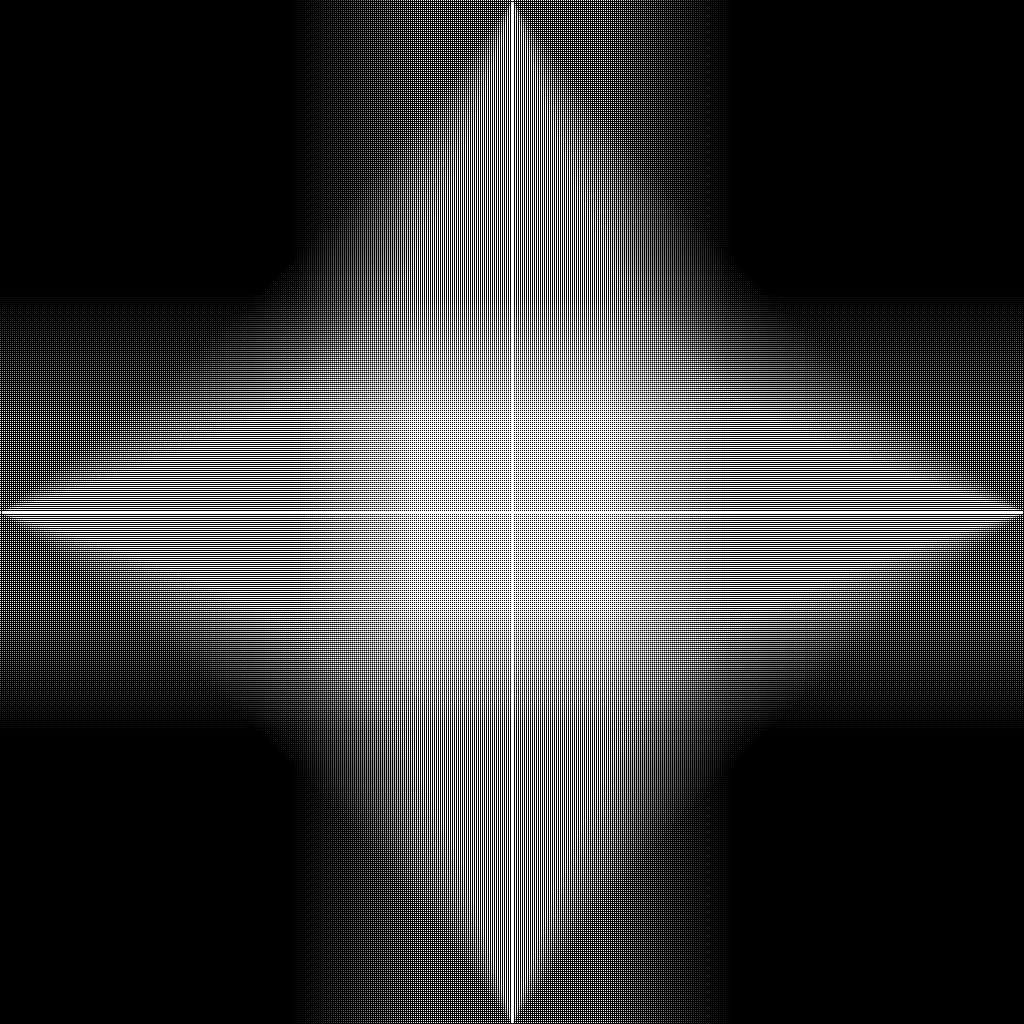
\includegraphics[width=.5\textwidth]{fig/out/6.img2_fft.png}
        \caption{Original shifted image}
    \end{subfigure}
    \begin{subfigure}{0.32\textwidth}
        \centering
        
\includegraphics[width=.5\textwidth]{fig/out/6.gaussian_filter_frequency.png}
        \caption{Gaussian filter for frequency domain}
    \end{subfigure}
    \begin{subfigure}{0.32\textwidth}
        \centering
        
\includegraphics[width=.5\textwidth]{fig/out/6.img2_filtered.png}
        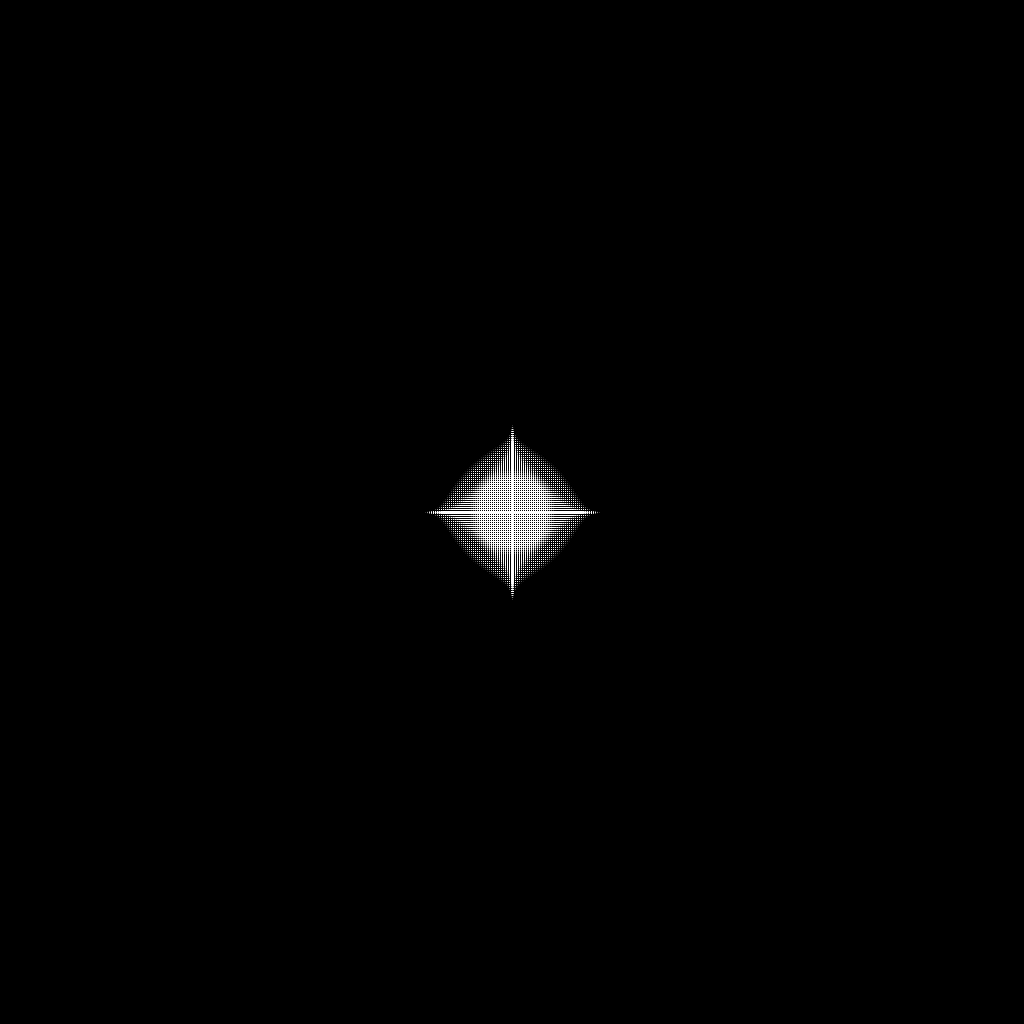
\includegraphics[width=.5\textwidth]{fig/out/6.img2_filtered_fft.png}
        \caption{Filtered image}
    \end{subfigure}
    \caption{Gaussian filtering pipeline in the frequency domain}
    \label{fig:ex6-frequency}
\end{figure}

\subsection{[BONUS] Benchmarking filtering pipelines in the spatial and frequency domain}
Let us now compare the two filtering pipelines in terms of execution time. We will vary the spatial sigma $\sigma_s$ and measure the execution time of both pipelines. Results are shown in \autoref{fig:ex6-benchmark}. We can see that the frequency domain filtering pipeline is faster than the spatial domain one for the majority of values of $\sigma_s$.\\\\
There are a couple of important remarks to make. We notice how the computational complexity of filtering in the frequency domain comes from computing the fourier spectrum of the image, and therefore depends on the size of the image, while the computational complexity of filtering in the spatial domain depends on the size of the kernel (and therefore on $\sigma$ in the case of gaussian filtering).\\Does this mean that for larger images spatial filtering is to be preferred ? Not necessarily. If an image has to be filtered multiple times (e.g in a image editing software), frequency filtering would require to compute the fourier spectrum only once, amortizing the computational cost over multiple filtering operations. Otherwise, when performing a single filtering operation on a very large image, spatial filtering would be preferred.
\begin{figure}[h!]
    \centering
\begin{tikzpicture}
    \begin{axis}[
      xlabel=Spatial sigma $\sigma_s$,
      ylabel=Execution time (seconds),
      legend pos=north west,
      ymajorgrids=true,
      grid style=dashed,
      height=10cm,
      width=\textwidth]
    \addplot table[x=x, y=y, mark=none] {./fig/out/6.benchmark.dat};
    \addplot table[x=x, y=z, mark=none] {./fig/out/6.benchmark.dat};
    \legend{Spatial filtering,Frequency filtering}
    \end{axis}
\end{tikzpicture}
\caption{Benchmark comparing Gaussian filtering in the spatial domain vs in the frequency domain}
\label{fig:ex6-benchmark}
\end{figure}



\clearpage
\section{Image Restoration [4 points]}
We are tasked in removing the checkerboard pattern from the provided image by cancelling out some frequencies in the fourier domain.
\begin{minted}[frame=lines, framesep=2mm, fontsize=\small ]{matlab} 
% ...
% Bring the image in the frequency domain
fft_img = fftshift(fft2(img));

% Compute the mask
mask = circleMask(size(img), 14, [210, 280]);
mask = mask + circleMask(size(img), 14, [265, 285]);
mask = mask + circleMask(size(img), 14, [215, 355]);
mask = mask + circleMask(size(img), 14, [270, 360]);
mask = ~mask;

% Apply the mask
fft_masked = fft_img .* mask;

% Unshift and bring in the spatial domain
fft_res = ifftshift(fft_masked);
img_res = ifft2(fft_res);
function mask = circleMask(imgsize, radius, position)
    [W,H] = meshgrid(1:imgsize(2),1:imgsize(1));
    mask = (((W-position(1)).^2 + (H-position(2)).^2) < radius^2);
end
\end{minted}
We notice how the checkerboard pattern is oriented diagonally. That is the clear indicator of a sum of equal sinusoids in both vertical and horizontal direction. In fact, the fourier spectrum of the image shows two peaks in both the horizontal and vertical direction. We can therefore cancel the pattern by masking the fourier spectrum in the corresponding frequencies. Results are shown in \autoref{fig:ex7}.
\begin{figure}[h!]
    \centering
    \begin{subfigure}{0.27\textwidth}
        \centering
        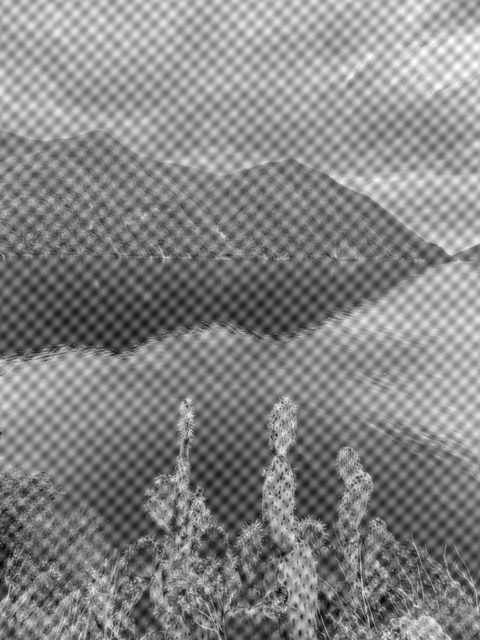
\includegraphics[width=.5\textwidth]{fig/out/7.img.png}
        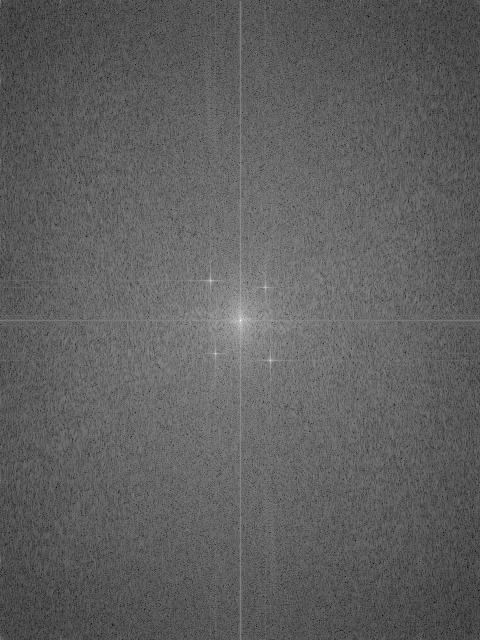
\includegraphics[width=.5\textwidth]{fig/out/7.img_fft.png}
        \caption{Original image}
    \end{subfigure}
    \begin{subfigure}{0.27\textwidth}
        \centering
        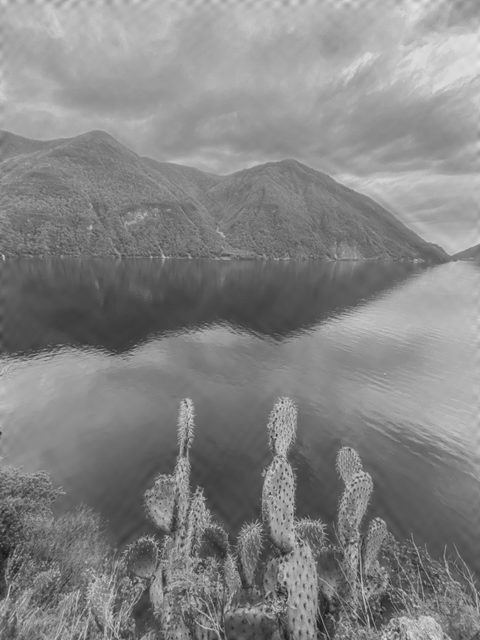
\includegraphics[width=.5\textwidth]{fig/out/7.res.png}
        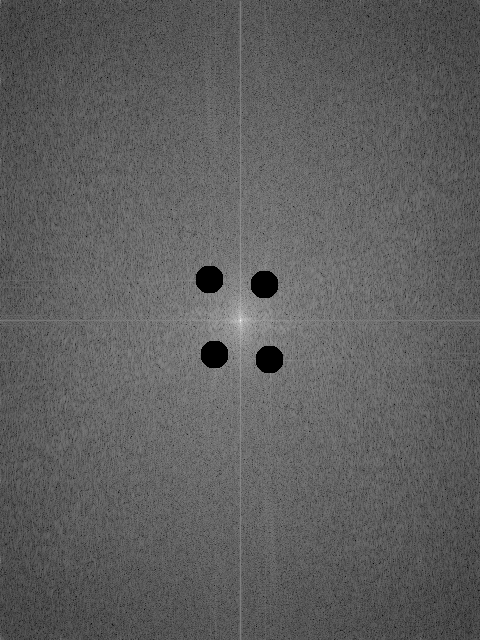
\includegraphics[width=.5\textwidth]{fig/out/7.res_fft.png}
        \caption{Image with masked pattern}
    \end{subfigure}
    \caption{Comparison of different histogram equalization techniques.}
    \label{fig:ex7}
\end{figure}


\section{Bonus}
Suppose an image is to be up-scaled by a factor of 2.
Firstly, the image is up-sampled as shown in \autoref{fig:ex6b}. The missing pixels can then be computed using two different interpolation methods: nearest neighbor (\autoref{fig:ex6c}) and linear interpolation (\autoref{fig:ex6d}).



\begin{figure}[H]
    \vspace*{-1cm}
    \centering
    \begin{subfigure}{0.24\linewidth}
        \centering
        \phantom{
\includegraphics[width=.5\linewidth]{./fig/out/8.cameraman_crop.png}}
        \raisebox{.5\height}{
\includegraphics[width=.5\linewidth]{./fig/out/8.cameraman_crop.png}}
        \caption{Original image}
        \label{fig:ex6a}
    \end{subfigure}
    \begin{subfigure}{0.24\linewidth}
        \centering
        
\includegraphics[width=\linewidth]{./fig/out/8.cameraman_up.png}
        \caption{Up-sampled image}
        \label{fig:ex6b}
    \end{subfigure}
    \begin{subfigure}{0.24\linewidth}
        \centering
        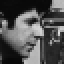
\includegraphics[width=\linewidth]{./fig/out/8.cameraman_nn.png}
        \caption{Nearest neighbor}
        \label{fig:ex6c}
    \end{subfigure}
    \begin{subfigure}{0.24\linewidth}
        \centering
        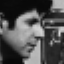
\includegraphics[width=\linewidth]{./fig/out/8.cameraman_l.png}
        \caption{Linear interpolation}
        \label{fig:ex6d}
    \end{subfigure}
    \caption{Up-scaling an image by a factor of 2.}
    \label{fig:ex6}
\end{figure}

The nearest neighbor method simply copies the value of the nearest pixel to the missing one. The method works by convolving the image with the following kernel:

$$\begin{bmatrix}
1 & 1 & 0 \\
1 & 1 & 0 \\
0 & 0 & 0 \\
\end{bmatrix}$$
Because of how the up-sampled image is constructed, if the pixel in the center of the kernel is present, the surrounding pixels will be missing and thus the resulting pixel will be the same as the center one. If instead the center pixel is missing, only one of the surrounding pixels will be present and thus used as the value of the missing pixel.


The linear interpolation method instead computes the value of the missing pixel as the weighted average of the four nearest pixels. The method works by convolving the image with the following kernel:
$$\frac14\begin{bmatrix}
    1 & 2 & 1 \\
    2 & 4 & 2 \\
    1 & 2 & 1 \\
\end{bmatrix}$$
If the pixel in the center of the kernel is present, the resulting pixel will be the same as the center one. If instead the center pixel is missing, the resulting pixel will be the weighted average of the four surrounding existing pixels in the corners or the mean of the two pixels at the sides if the corner pixels are missing as well.

\autoref{fig:ex8-intensitiesplot} shows the signal of a single row of the up-scaled image with the two methods. Because of linear interpolation, the linearly interpolated signal is the same as the original one, just stretched by a factor of 2. The nearest neighbor method instead results in a more noisy signal since the missing pixels are simply copied from the nearest existing ones, while in linear interpolation the pixel intensities follow a smoother curve.\\
In the Fourier domain (\autoref{fig:ex8-fourierplot}) this results in the image up-scaled with nearest neighbor interpolation having more high frequencies while the image up-scaled with linear interpolation has the same frequencies as the original image.
Thus, the ratio between the Fourier transforms of the linear interpolation up-scaled image and the nearest-neighbor up-scaled image will be close to 1 on lower frequencies (i.e the spectrums are almost identical) and will decrease for higher frequencies (i.e. the spectrum of the linearly interpolated image will have more energy on higher frequencies). This is confirmed by the plot in \autoref{fig:ex8-fourierplot}. Intuitively, it can be seen from the upscaled images that the linearly interpolated image is smoother than the nearest neighbor one, thus having less high frequencies.

\begin{figure}[h!]
    \centering
\begin{tikzpicture}
    \begin{axis}[
      xlabel=Pixel position $x$ in the image row,
      ylabel=Intensity $I$,
      legend pos=north west,
      ymajorgrids=true,
      grid style=dashed,
      height=10cm,
      width=\textwidth]
    \addplot table[x=x, y=y, mark=none] {./fig/out/8.intensities.dat};
    \addplot table[x=x, y=z, mark=none] {./fig/out/8.intensities.dat};
    \legend{Nearest Neighbor,Linear Interpolation}
    \end{axis}
\end{tikzpicture}
\caption{Pixel intensities for one image row of the two interpolation methods.}
\label{fig:ex8-intensitiesplot}
\end{figure}

\begin{figure}[h!]
    \centering
\begin{tikzpicture}
    \begin{axis}[
      xlabel=Frequency $\omega$,
      ylabel=Gain $A$,
      legend pos=north west,
      ymajorgrids=true,
      grid style=dashed,
      height=10cm,
      width=\textwidth]
    \addplot table[x=x, y=y, mark=none] {./fig/out/8.fourier.dat};
    \addplot table[x=x, y=z, mark=none] {./fig/out/8.fourier.dat};
    \legend{Nearest Neighbor,Linear Interpolation}
    \end{axis}
\end{tikzpicture}
\caption{Fourier plot of the two interpolation methods.}
\label{fig:ex8-fourierplot}
\end{figure}




\end{document}